% Chapter Template

\chapter{Literature Review} % Main chapter title

\label{chap:Chapter10} % Change X to a consecutive number; for referencing this chapter elsewhere, use \ref{ChapterX}

It has long been a desire of mankind to know what occurs at the cellular level. Even to get the smallest glimpse of this world would have been extremely rewarding. This was made possible in the 1670s by Antoni van Leeuwenhoek when he took the first steps to build a microscope \cite{Meijering2012}. The field of cellular biology has rapidly expanded ever since.
In more recent times, the fluorescent microscope has allowed biologists and other professionals alike to not only restrict their studies to cellular and subcellular organisms in great detail, but also to store the data in images and videos. This stored data allows scientists to critically analyse and reanalyse the same data to get the most information out of it. As a result, there is a titanic-size volume of image data to be analysed.
The image data is so abundantly variant in heterogeneity, dimensionality, complexity and quality such that manual image processing and analysis cannot keep up in terms of time and quality \cite{Meijering2012}. Most of the useful cell analysis starts at the cell segmentation level and this is a major bottleneck, in time and quality, that needs to be avoided.\\


\begin{definition}[What has fluorescence image segmentation been through?]
	Machine assistance in fluorescence image segmentation is not new and dates as far back as the mid-1950s where thresholding on serialised (1D) data was done to enable mass screening for cervical cancer \cite{Tolles1955}. Since then, biologists, and other professionals alike, began to rely heavily on computerised image segmentation of cells.
	A timeline of the major advancements in segmentation and cell segmentation is shown in \autoref{fig:literaturereviewtimeline}.
	
	The shift from 1D image processing to 2D image processing happened in the early 1960s \cite{Prewitt1966} and was still threshold-based.
	It wasn't until the mid-1960s where feature segmentation and mathematical morphology was tested on fluorescence image data \cite{Prewitt1966,David1967}.
	Thresholding still dominated up until the mid-1970s; when research focus shifted to morphological segmentation \cite{Greipp1976}. 
	It was also the time when researchers in image processing started to get more interested in fluorescence image processing and started to try out other techniques such as those based on Random Fields \cite{Banks1975}.
	None of the emerging techniques worked well enough with the problems posed in fluorescence imaging until the late 1970s when the Watershed method was used \cite{Beucher1979}.
	Watershed segmentation began to gain a lot of momentum in comparison to the other new techniques but thresholding was still the technique of preference due to it's, by then, long history.
	At the same time, variants of thresholding became the new focus of cell segmentation. This started with the histogram thresholding method \cite{hoffman1984} in 1984 and then Otsu segmentation \citep{Geerts1988} in 1988.
	
	\begin{figure}[!t]
		\centering
		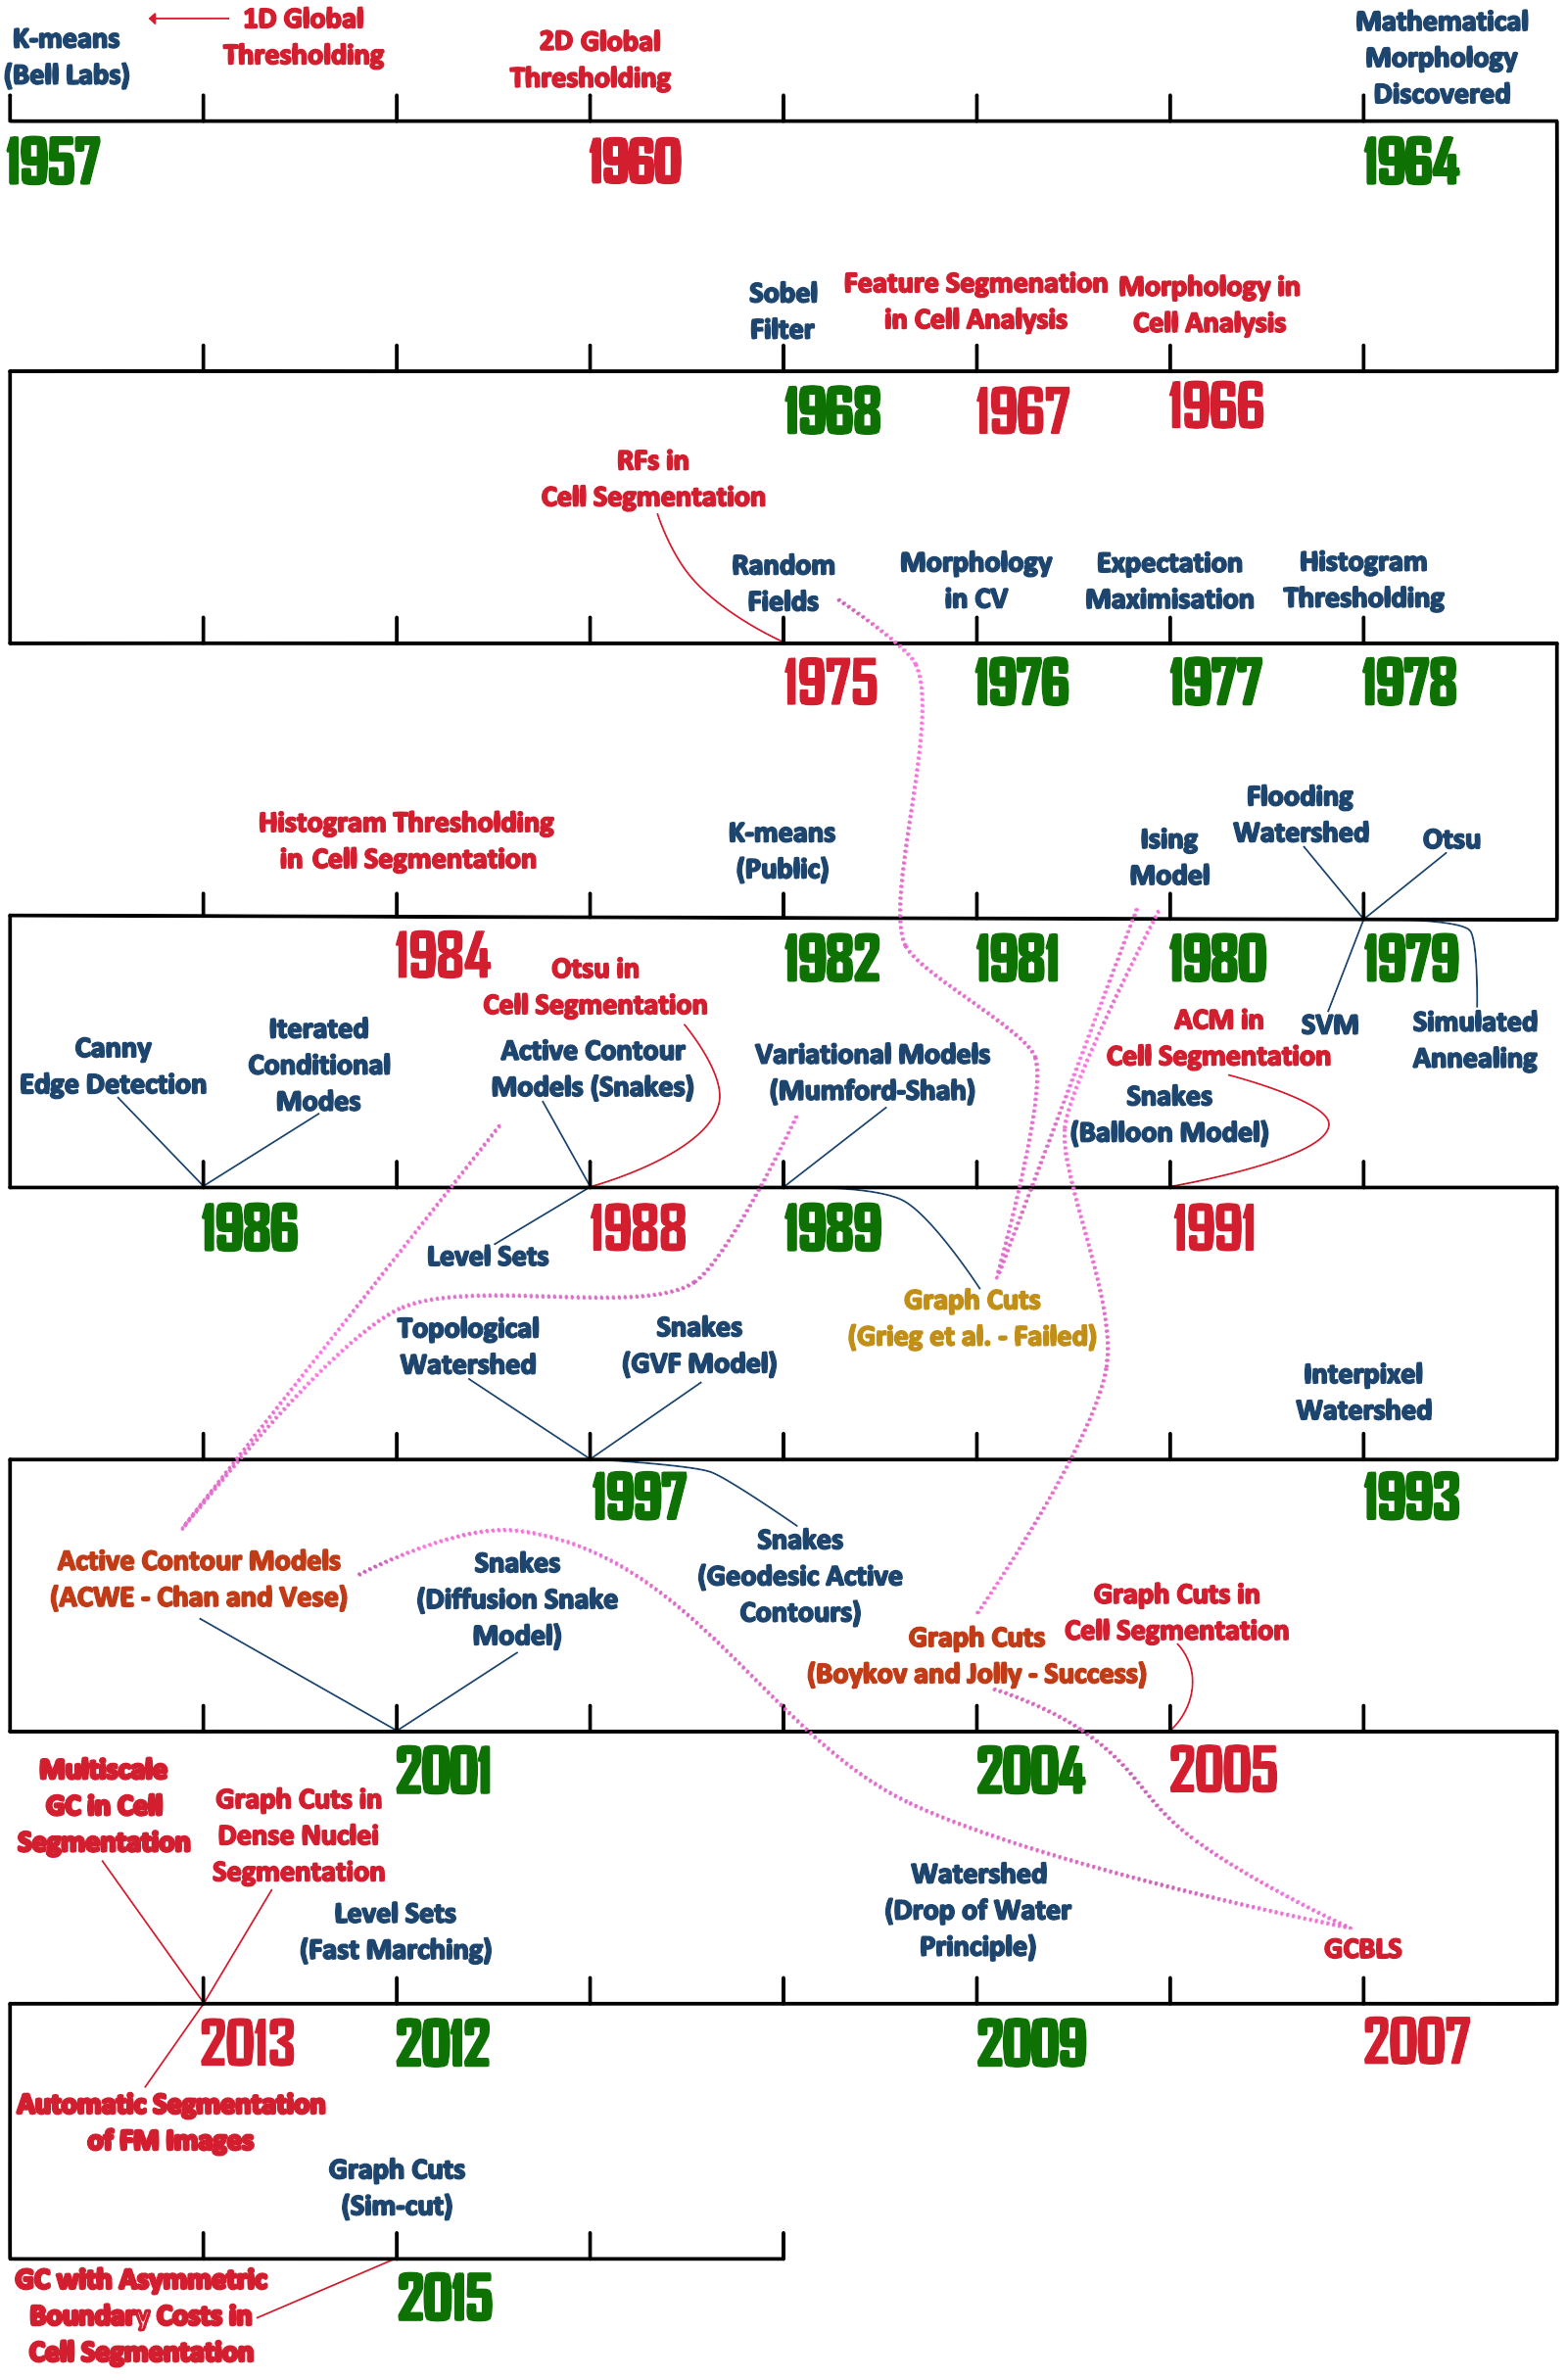
\includegraphics[width=0.93\columnwidth]{literature_review.png}
		\caption{Progression of cell segmentation techniques. Text in red highlight momentous advancements fluorescence image segmentation of cells.}
		\label{fig:literaturereviewtimeline}
	\end{figure}
	
	Much of the segmentation techniques developed were very algorithmically simple with little computational demand. This was because computational power was a rare resource. This ended in 1990 when computational power rapidly increased and continued to increase. This made it possible for more sophisticated and computationally demanding techniques to be implemented in fluorescence image segmentation; such as Active Contour Models (ACM) \cite{Samarabandu1992} in 1992.
	It was also a time when more morphologically accurate segmentations where required and the previous methods really began to fall short of the required expectations. Cellular biologist, and other professional alike, demanded segmentation of specific objects of interest such as cell nuclei, chromosomes, other specific proteins, etc. It was not until 2005 that Graph Cuts (GC), our technique of focus in this dissertation, began to appear on the cell segmentation scene \cite{Baggett2005}.\\
	
	Although the challenges in fluorescence image segmentation are very unique to the field, there has not been any segmentation techniques developed to exclusively handle fluorescence images \cite{Meijering2012}. The techniques used in FM segmentation have always been ported from techniques that were designed to segment other types of data. Segmentation techniques in fluorescence imaging seem to follow other segmentation schemes rather than lead or plot its own course.
	This can be seen in the timeline in \autoref{fig:literaturereviewtimeline} where, in 1966, mathematical morphology was used in cell segmentation although it had been discovered two years prior. Similarly, the case for the application of Otsu binarization in cell segmentation is even worse with its first application to the field in 1988 \citep{Geerts1988}, although it had been designed in 1979 \cite{Otsu1979}.
	
	On the other hand, rather than embracing newer techniques, the field of fluorescence image analysis is reluctant to accept the modern and sophisticated techniques. Consequently, most of the fluorescence image segmentation done today uses thresholding methods, watershed techniques, feature detection like edge detection, and region accumulation \cite{Meijering2012}. However, this has not hindered research and regular progress of applying the more sophisticated segmentation models to fluorescence images. Fortunately, modern segmentation methods are increasingly gaining momentum and becoming the method of preference as of late.
\end{definition}


% Borgefors1986
% Peng2009
% Russel2009
% Du2010
% Dima2011
% Smochina2011
% Anielski2012
% Yang2013
% Hu2013
% Qi2013
% Hossain2013
% Ghaye2013
% Preethi2014
% Fatichah2014
% Raza2015

\begin{definition}[Where is fluorescence image segmentation now?]
	We now focus on the relevant research in the last decade. Much of the research involves combining many segmentation methods or designing a variant of an existing method to eliminate a certain problem \cite{Smochina2011,Meijering2012}. These solutions also tend to be very isolated to the specific problem and resultantly suffer from diminished diversity of application.\\
	
	In 2009, Peng and Hsu \cite{Peng2009} designed a variant of adaptive local thresholding flor fluorescence cell micrographs. This was to combat the varying brightness and contrast throughout the image. They compared their technique against Otsu binarization \cite{Otsu1979}, Iterative thresholding method \cite{Ridler1978}, Niblack's thresholding method \cite{Niblack1986} and the then recent adaptive thresholding based on the variational minmax algorithm \cite{Saha2009}. Most of these are very old techniques whose weaknesses are well-known. Also, although their experiments did involve images with significant brightness and contrast issues, all the images are very similar. Their segmentation was not automatic, it did require manual tuning and no process or discussion was given on how they had arrived at their parameters. In their efforts to replace manual segmentation with automatic segmentation, they've instead diverted to a parameter tuning problem; which is just as time consuming.
	
	A similar situation is seen when Du \textit{et al.} \cite{Du2010}, in 2010, published their performance evaluation studies by comparing K-means, Otsu, EM and Global Minimisation of the Active Contour Model (GMAC) on fluorescence microscopy cell images. They had used a combination of synthetic and real data and concluded that GMAC performed the best overall. However, no mention was given as to how some of the parameter values were chosen for GMAC. Considering that the performance improvement by GMAC was slightly better that K-means and Otsu, it would be better to use any of the latter techniques, instead of playing around with parameters for a slight improvement when using GMAC.
	
	In 2011, Dima \textit{et al.} \cite{Dima2011} compared several commonly used algorithms in fluorescence image segmentation using their novel biviarate similarity index. They had concluded that K-means and Canny edge detection is superior to Otsu, maximum entropy and isodata. However, they had used very simple images.
	
	In 2012, Alexander \textit{et al.} \cite{Anielski2012} designed an image segmentation scheme which was designed around global thresholding. They ended up with a hard-coded number to be used in their global thresholding method. If history is any indication, then this has extremely limited use and will fall away in the "not-so-long" term. Research into fluorescence image segmentation has almost guaranteed that there is no "magic number". Instead we seek a method that is flexible enough to accommodate the variation of fluorescence images and still deliver a consistent and expected output.
	
	In 2013, there was an explosion of published material of fluorescence image segmentation. This was accompanied by significant application of graph cut segmentation in the domain. Qi \cite{Qi2013} designed a novel segmentation scheme combining graph cuts and the convex shape assumption. The proposed initialisation was based on the Poisson model of intensity for FM images. Upon initialisation, a standard graph cut algorithm would perform the segmentation. He used the Boykov and Funka-Lea energy functions \cite{Boykov2006}.
	Afterwards, he performs convexity analysis to split overlapping or touching cell nuclei. This was a successful attempt and proved the ability of graph cuts to handle fluorescence images. His scheme outperformed the Watershed method, both direct and gradient variants, Otsu, Mean threshold, Active masks, Merging algorithm, RC threshold and AS threshold. He also tested on a large dataset of 78 images each of size 1940 $\times$ 1940. The performance was based on the Hausdorff distance. However, he was unable to get rid of the parameter tuning required for that energy function, $\lambda$, which controls the relative importance or regional and boundary terms.
	
	In the same year, graph mining was pitted against Supervised machine learning segmentation, Support Vector Machines (SVM) \cite{Hossain2013}. Graph mining ended with an 85\% accuracy beating SVMs which had a 72\% accuracy. The process involves a pre-processing scheme of Gaussian noise removal and background removal by thresholding. Their experiments were done over a small set of 10 images. Moreover, no images nor image segmentation mask or contours were published. One would have to assume that there is limited variation of fluorescent embryonic stem cell images for it to be left out.
	
	In 2014, Preethi \textit{et al.} \cite{Preethi2014} proposed an automatic segmentation and tracking scheme of fluorescent cancerous cells by Wavelet Otsu model. The scheme involved a pre-process of adaptive histogram equalisation (AHE) and anisotropic diffusion filtering. They used morphological techniques to track cell shape. However, they have not published any object results and no comparison to state-of-the-art or other leading techniques.
	
	In 2015, Raza \textit{et al.} \cite{Raza2015} proposed a novel automatic segmentation technique by combining textural information in the wavelet domain to counteract the variable intensity in FM images. They tested their technique against active contours \cite{Bergeest2012} and supervised template matching \cite{Chen2013}. They compared the algorithm on various performance measures. On most measures the proposed system outperformed the competitor methods.
\end{definition}

\begin{definition}[Where is fluorescent image segmentation heading?]
	From the recent research and publications, it seems as if there is a new technique designed to work on each sub-field in which fluorescence images are attained. Instead of converging to a unified solution, there seems to be a divergence that is getting increasingly stronger.
	Many of the novelties are schemes involving a pre-process and following segmentation technique. 
	
	Many solutions also involve manual parameter tuning. There is also a lack of published methodologies for parameter tuning in these schemes.
	
	One can conclude that there is a diverging number of solutions for fluorescence image segmentation.
	
	What is needed, is a segmentation method that performs consistently and delivers expected results on a large diversity of fluorescence images that minimises user-interaction. Ideally, it would eliminate user-interaction.
\end{definition}












